% This must be in the first 5 lines to tell arXiv to use pdfLaTeX, which is strongly recommended.
\pdfoutput=1
% In particular, the hyperref package requires pdfLaTeX in order to break URLs across lines.

\documentclass[11pt]{article}
% 1) Include xcolor with the [table] option so cell coloring works.
\usepackage[table]{xcolor}

% 2) Include soul so \hl and \sethlcolor work.
\usepackage{soul}

% 3) Define any custom colors you actually use in the table.
\definecolor{pastelyellow}{rgb}{1.0, 1.0, 0.8}
\definecolor{lightgray}{gray}{0.92}
\definecolor{teagreen}{rgb}{0.82, 0.94, 0.75}
\definecolor{pinksecondbest}{rgb}{1.0, 0.82, 0.86}
\definecolor{pastelviolet}{rgb}{0.87, 0.81, 0.96}
\definecolor{predcolor}{rgb}{1.0, 0.86, 0.85}
% Remove the "review" option to generate the final version.
\usepackage{ACL2023}

% Standard package includes
\usepackage{times}
\usepackage{latexsym}
\usepackage{graphicx}      % For including images
\usepackage{amsmath}       % For better math support (like align, etc.)
\usepackage{amssymb}       % For symbols like ℝ
\usepackage{mathtools}     % For extended math functionality
\usepackage{caption}       % For better figure captions
\usepackage{hyperref}      % For hyperlinks
\usepackage{cleveref}      % For \Cref-style references

% For proper rendering and hyphenation of words containing Latin characters (including in bib files)
\usepackage[T1]{fontenc}
% For Vietnamese characters
% \usepackage[T5]{fontenc}
% See https://www.latex-project.org/help/documentation/encguide.pdf for other character sets

% This assumes your files are encoded as UTF8
\usepackage[utf8]{inputenc}

% This is not strictly necessary, and may be commented out.
% However, it will improve the layout of the manuscript,
% and will typically save some space.
\usepackage{microtype}

% This is also not strictly necessary, and may be commented out.
% However, it will improve the aesthetics of text in
% the typewriter font.
\usepackage{inconsolata}


% If the title and author information does not fit in the area allocated, uncomment the following
%
%\setlength\titlebox{<dim>}
%
% and set <dim> to something 5cm or larger.

\title{Parameter-Efficient Transfer Learning of Audio Spectrogram Transformers}

% Author information can be set in various styles:
% For several authors from the same institution:
% \author{Author 1 \and ... \and Author n \\
%         Address line \\ ... \\ Address line}
% if the names do not fit well on one line use
%         Author 1 \\ {\bf Author 2} \\ ... \\ {\bf Author n} \\
% For authors from different institutions:
% \author{Author 1 \\ Address line \\  ... \\ Address line
%         \And  ... \And
%         Author n \\ Address line \\ ... \\ Address line}
% To start a seperate ``row'' of authors use \AND, as in
% \author{Author 1 \\ Address line \\  ... \\ Address line
%         \AND
%         Author 2 \\ Address line \\ ... \\ Address line \And
%         Author 3 \\ Address line \\ ... \\ Address line}

\author{Eltar Mazoz \\
  Tel Aviv University \\
  \texttt{eltarmazuz@mail.tau.ac.il} \\\And
  Omer Talmi \\
  Tel Aviv University \\
  \texttt{omertalmi@mail.tau.ac.il} \\}

\begin{document}
\maketitle
\begin{abstract}

\end{abstract}

\section{Introduction}


\section{Related Work}
One of the big breakthroughs in deep learning for vision tasks was the introduction of the Vision Transformer (ViT) \cite{dosovitskiy2020image}, which builds upon the transformer architecture \cite{vaswani2017attention}. Unlike convolutional neural networks (CNNs), ViT processes images as sequences of patches, leveraging self-attention mechanisms to model long-range dependencies across an image. This shift in paradigm has led to competitive or superior performance compared to CNNs, especially when trained on large datasets. ViT’s success has also extended beyond vision, inspiring models such as the Audio Spectrogram Transformer (AST) for audio classification, demonstrating the versatility of transformer-based architectures in various modalities \cite{gong2021ast}.


\section{Method}
\subsection{Overview of Parameter-efficient Transfer Learning Methods}

We now introduce the PETL techniques we used in our experiments: LoRA, Pref-T 24, Linear probing, adapter tuning, and full fine-tuning.
We also introduce our novel method to use freq-LoRA for finetuning AST.

\subsubsection{Full Fine-Tuning}
Full fine-tuning (FFT) adapts the entire pre-trained model to each downstream task \cite{xu2023parameter}. This approach ensures optimal performance by adjusting all model parameters, but it requires significant computational resources and storage. Fine-tuning the full model is often impractical for resource-constrained environments, particularly in multi-task learning scenarios where maintaining separate models for each task becomes infeasible.

\subsubsection{Pref-T 24 (Prefix-Tuning)}
Prefix-tuning inserts a set of $p$ learnable continuous embeddings of dimension $d$ (i.e., prompts) into the keys and values of the MHSA block at every layer \cite{li2021prefix}. Pref-T 24 follows the deep prompt-tuning (DPT) paradigm, where prompts are uniformly prepended to each transformer layer instead of just the first layer, as in shallow prompt-tuning (SPT). By strategically placing the prefix embeddings throughout the network, Pref-T 24 enhances the model’s ability to generalize across tasks while maintaining parameter efficiency.

\subsubsection{Linear Probing}
Linear probing is a lightweight fine-tuning method where only the classification head (i.e., the final linear layer) of the pre-trained model is updated, while the rest of the model remains frozen \cite{kumar2022finetuning}. This approach significantly reduces computational cost and prevents catastrophic forgetting by preserving the original model’s learned representations.

Given an input sequence $X_{\text{in}}$, the output of the frozen transformer layers is represented as:

\begin{equation}
X_{\text{out}} = \text{Transformer}(X_{\text{in}})
\end{equation}

A task-specific linear classification head $W_{\text{lin}} \in \mathbb{R}^{d \times C}$, where $C$ is the number of output classes, is then applied to obtain the final predictions:

\begin{equation}
\hat{y} = X_{\text{out}} W_{\text{lin}}
\end{equation}

Although linear probing is highly efficient and requires only a small number of trainable parameters, its performance is often inferior to other PETL methods such as LoRA or adapter-based tuning, especially for tasks requiring deeper model adaptation. Its effectiveness strongly depends on the quality and task-relevance of the representations produced by the foundation model. Nevertheless, linear probing remains a strong baseline for transfer learning scenarios where computational resources are limited.

\subsubsection{LoRA (Low-Rank Adaptation)}
LoRA introduces trainable low-rank matrices into transformer layers to approximate the weight updates \cite{hu2021lora}. For a pre-trained weight matrix $W \in \mathbb{R}^{d \times d_k}$, LoRA represents its update with a low-rank decomposition $W + \Delta W = W + AB$, where $A \in \mathbb{R}^{d \times r}$, $B \in \mathbb{R}^{r \times d}$, and $r \ll d$. LoRA typically applies this update to the query and value projection matrices, $W_q$ and $W_v$, in the Multi-Head Self-Attention (MHSA) sub-layer. The computation of query and value matrices follows:

\begin{equation}
Q/V = X_{\text{in}} W_{q/v} + s \cdot X_{\text{in}} A_{q/v} B_{q/v}
\end{equation}

where $s$ is a tunable scalar hyperparameter. This method allows efficient adaptation of the pre-trained model by introducing a minimal number of trainable parameters, thereby reducing storage requirements.

\subsubsection{Conformer Adapter: Pfeiffer Configuration}
Adapters are small, trainable modules inserted into transformer layers \cite{he2021towards}. They employ a bottleneck structure to minimize additional parameters while still enabling task-specific adaptation. Specifically, the hidden representation of dimension $d$ is first down-projected to a smaller dimension $r$, then passed through a non-linear transformation, and finally up-projected back to $d$. Formally, for a transformer layer output $X_{\text{FF}}$ from the feed-forward (FF) block and a residual connection $X̂$, the Pfeiffer configuration places an adapter \emph{after} the FF block:
\begin{equation}
X_{\text{out}} \;=\; X̂ \;+\; X_{\text{FF}} \;+\; f\bigl(X̂\,W_{\text{down}}\bigr)\,W_{\text{up}},
\end{equation}
where $W_{\text{down}} \in \mathbb{R}^{d \times r}$ and $W_{\text{up}} \in \mathbb{R}^{r \times d}$, and $f(\cdot)$ is a non-linear activation function (e.g., ReLU). 

\paragraph{Motivation for Integrating Convolution.}
While a purely linear bottleneck adapter can be effective, it may struggle to capture local and contextual information in speech or audio tasks. Hence, a lightweight convolution module inspired by Conformer, retaining the Pfeiffer placement scheme to keep the number of additional parameters low.

To better model local dependencies while preserving the bottleneck design, replacing the simple down-up linear layers with a \textbf{depthwise convolution} module from the Conformer architecture. This design greatly enhances performance on speech and audio tasks:

\begin{enumerate}
    \item \textbf{Pointwise Down Convolution}: The input $X̂$ is projected to a hidden dimension of $2r$. 
    \item \textbf{Gated Linear Unit (GLU)}: This reduces the projected feature size to $r$.
    \item \textbf{Depthwise Convolution}: A depthwise convolution of kernel size $k$ is applied, followed by Batch Normalization and a Swish activation function. This efficiently captures local patterns with minimal extra parameters.
    \item \textbf{Pointwise Up Convolution}: Finally, we project the hidden representation back to dimension $d$.
\end{enumerate}

Placed after the FF block (as in Pfeiffer), the Conformer Adapter can significantly improve performance on challenging audio or speech tasks.
\begin{figure}[ht]
    \centering
    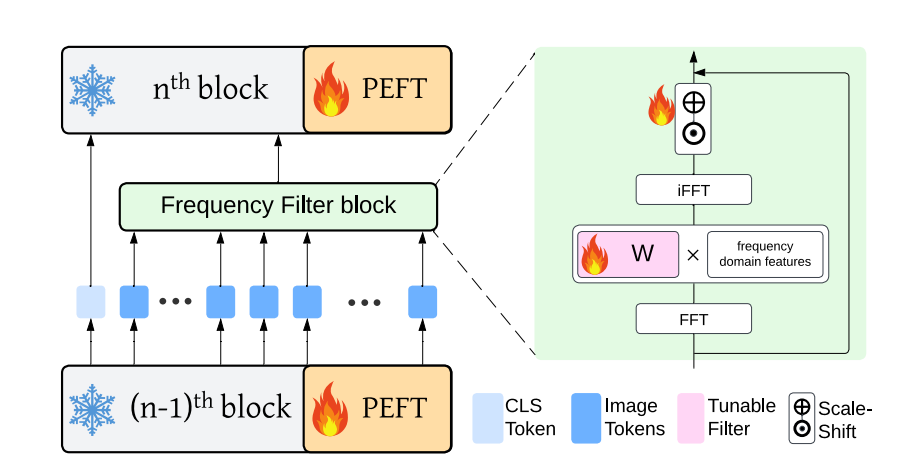
\includegraphics[width=1.2\linewidth]{freq_image.png}
    \caption{Illustration of the Freq-LoRA architecture. The method first applies LoRA, followed by a learnable frequency-domain transformation using FFT, complex-valued filtering, and inverse FFT, plus scaling-shifting and residual addition.}
    \label{fig:freq-lora}
\end{figure}

\subsubsection{Freq-LoRA (Frequency-Aware Low-Rank Adaptation)}

Freq-LoRA is a novel fine-tuning method that combines the efficiency of low-rank adaptation with the spectral modulation capabilities of frequency-domain feature transformation. Building upon LoRA's decomposition of pre-trained weight matrices into low-rank trainable components \cite{hu2021lora}, Freq-LoRA further enhances model expressiveness by injecting a frequency-based transformation module, inspired by FreqFit \cite{ly2024enhancing}, between transformer blocks. As shown in \Cref{fig:freq-lora}, the method first applies standard LoRA updates to the query and value projections within the multi-head self-attention sublayer, then modulates the resulting hidden representations in the frequency domain using a learnable complex-valued filter. This is followed by an inverse FFT and a learnable scaling-shifting operation, which is added back via a residual connection. Formally, for an input representation $X \in \mathbb{R}^{B \times N \times d}$, Freq-LoRA computes:

\begin{equation} \hat{X} = \text{IFFT}(K \odot \text{FFT}(X)) \cdot \alpha + \beta + X \end{equation}

where $K$ is a learnable complex-valued filter, and $\alpha, \beta \in \mathbb{R}^d$ are learnable scale and shift parameters. This integration allows Freq-LoRA to capture both spatial and spectral dependencies, improving the model's ability to adapt to fine-grained patterns and high-frequency information. Extensive empirical results show that Freq-LoRA outperforms baseline LoRA and other PEFT methods across a variety of tasks, especially in low-resource or domain-shifted scenarios.

\begingroup
\setlength{\tabcolsep}{3.3pt}
\newcolumntype{K}{!{\color{white}\ }c}

\begin{table}[t]
\centering
\caption{Performance evaluations of the PETL methods on ESC and US8K for AST. 
Best and second-best performances for each dataset are coloured in 
\sethlcolor{teagreen}\hl{\textbf{Green}} and 
\sethlcolor{pinksecondbest}\hl{Red}, respectively.}
\label{tab:main}
\begin{tabular}{lKKK}
\toprule
\textbf{Method} & \textbf{Par} & \cellcolor{pastelyellow}\textbf{ESC} & \cellcolor{lightgray}\textbf{US8K}\\
\midrule
FFT &  85M & \cellcolor{pinksecondbest}87.50 & \cellcolor{teagreen}\textbf{83.08}\\
Linear     & 9/40K   & 74.64      & 76.67\\
\hline \addlinespace
Pref-T 24  & 221K    & 82.75      & 81.11\\ 
LoRA       & 221K    & 85.80      & \cellcolor{pinksecondbest}84.12\\
\hline
\rowcolor{pastelviolet}
\multicolumn{4}{l}{\textbf{Conformer Adapter}}\\
\hline \addlinespace
Pfeiffer   & 271K    & \cellcolor{teagreen}87.30 & 81.60\\
\bottomrule
\end{tabular}
\end{table}
\endgroup


\section{Experiments}
\subsection{Implementation Details}

\textbf{Datasets}. We evaluate the PETL methods on two widely used environmental sound classification benchmarks: ESC-50 and UrbanSound8K (US8K). ESC-50 (ESC) \cite{piczak2015esc} consists of 2,000 five-second-long audio recordings spanning 50 everyday acoustic events (e.g., dog barking, footsteps). US8K \cite{salamon2014dataset} includes 8,732 short audio excerpts (up to four seconds each) from 10 urban sound categories (e.g., sirens, drilling). Both datasets present significant background noise and intra-class variability, making them suitable for evaluating model robustness and generalization.

\textbf{Evaluation Metric}. We use classification accuracy as the primary evaluation metric, defined as:
\begin{equation}
    \text{Accuracy} = \frac{\text{Number of correct predictions}}{\text{Total number of predictions}}.
\end{equation}

\textbf{Validation Protocol}. For ESC-50, we use 5-fold cross-validation and report the average accuracy across the folds. For US8K, we follow the standard protocol and evaluate using 3 folds instead of the 10 official folds, because of computation limits,  and report the average accuracy across the folds. In $k$-fold cross-validation, the dataset is divided into $k$ equal parts; the model is trained on $k-1$ parts and tested on the remaining part, iteratively, ensuring each part is used as a test set exactly once.



\textbf{Computational Setup and Challenges.} Initially, we trained our models using the university's SLURM-based cluster. However, due to memory constraints, we had to significantly reduce the batch size to fit the model into the available resources. This led to suboptimal convergence and degraded performance. To overcome these limitations, we migrated to Google Colab with an A100 GPU, allowing for larger batch sizes and more stable training. Nonetheless, the performance remained unsatisfactory until we carefully tuned the Reduction Ratio (RR) of the adapters. We observed that increasing RR from 64 to 96 significantly improved accuracy, suggesting that higher compression levels helped regularize the model and reduce overfitting. This highlights the importance of proper RR selection when applying PETL methods to AST-based models.



\section*{Limitations}

\section*{Acknowledgements}

We would like to thank our lecturer, Tal Rosenwein Kariboy
, for introducing us to deep learning and deep learning on audio processing. The methods we learned in this course have already proven useful in other domains we work in. We are grateful for your dedication and effort throughout the course.


\subsection{References}
\bibliographystyle{ACM-Reference-Format}
\bibliography{custom}



\end{document}
